\documentclass[11pt,a4paper]{article}

% --- Pakker ---
\usepackage[utf8]{inputenc}
\usepackage[T1]{fontenc}
\usepackage[danish,provide=*]{babel}
\usepackage{amsmath, amssymb}
\usepackage[a4paper, margin=2.2cm]{geometry}
\usepackage{tikz}
\usepackage{pgfplots}
\pgfplotsset{compat=1.18}
\usetikzlibrary{arrows.meta,decorations.markings,calc,patterns}
\usepackage{booktabs}
\usepackage{enumitem}
\usepackage{xcolor}
\usepackage{wasysym}
\usepackage{hyperref}

\hypersetup{
  colorlinks=true,
  linkcolor=blue!50!black,
  urlcolor=blue!50!black
}

% Farver (BasedNode-stemning)
\definecolor{bgpurple}{HTML}{7C5CFC}
\definecolor{bgcyan}{HTML}{38BDF8}
\definecolor{bgink}{HTML}{0B0D17}
\definecolor{bgorange}{HTML}{F0A419}

% --- Opgave-makro (Titel + indhold) ---
\newcommand{\opg}[2]{%
  \par\vspace{0.7em}\noindent
  \textbf{\large #1}\par
  #2\par
}

% --- Facit (bruges kun i appendix) ---
\newcommand{\f}[2]{%
  \par\vspace{0.35em}\noindent\textbf{Opgave #1:}\ #2\par
}

% --- Regel-boks (forklaring) ---
\newcommand{\regel}[2]{%
  \par\vspace{0.4em}\noindent
  \begin{tikzpicture}
    \node[draw=bgcyan!70, fill=bgcyan!10, inner sep=8pt,
          text width=\linewidth-2\fboxsep-2\pgflinewidth-9pt, align=left]
          {\textbf{Regel:} #1\\[2pt]\textit{#2}};
  \end{tikzpicture}\par
}

% --- Eksempel-boks (fuldt udregnet) ---
\newcommand{\eksempel}[2]{%
  \par\vspace{0.3em}\noindent
  \fcolorbox{bgink!30}{yellow!6}{%
    \parbox{0.96\linewidth}{%
      \textbf{Eksempel:}\ \textit{#1}\\[3pt]
      #2
    }%
  }\par
}

% --- Tipboks (hjælpende tekst i opgaven) ---
\newcommand{\tipbox}[1]{%
  \par\vspace{0.3em}\noindent
  \begin{tikzpicture}
    \node[draw=bgpurple!70, fill=bgpurple!8, inner sep=6pt,
          text width=\linewidth-2\fboxsep-2\pgflinewidth-9pt, align=left]
          {\textit{Tip:} #1};
  \end{tikzpicture}\par
}

% --- Crashes-boks (hvad sker der intuitivt) ---
\newcommand{\crash}[1]{%
  \par\vspace{0.3em}\noindent
  \begin{tikzpicture}
    \node[draw=bgpurple!80, fill=bgink!3, rounded corners=4pt, inner sep=8pt,
          text width=\linewidth-2\fboxsep-2\pgflinewidth-9pt, align=left]
          {\textbf{\color{bgpurple}Crash-forklaring:}\\[2pt]#1};
  \end{tikzpicture}\par
}

% --- Plot-hjælper: brøkvisualisering (lagkage / andel) ---
\newcommand{\fractionplot}[4]{%
% #1 = tæller (heltal), #2 = nævner (heltal), #3 = label farve, #4 = tekst
\begin{center}
\begin{tikzpicture}
  % Vandret bjælke delt i #2 lige store dele, #1 er udfyldt (én enkelt fyld-kommando)
  \draw[bgink!30, thin] (0,0) rectangle (10,0.7);
  \foreach \i in {1,...,#2} {
    \draw[bgink!50, thin] ({10*\i/#2},0) -- ({10*\i/#2},0.7);
  }
  \fill[bgpurple!70] (0,0) rectangle ({10*#1/#2},0.7);
  % Brøklabel under
  \node[bgink] at (5,-0.5) {\Large$\dfrac{#1}{#2}$};
  \node[bgink!80] at (5,-1.0) {\small #4};
\end{tikzpicture}
\end{center}
}

% --- Plot-hjælper: søjlediagram (hyppighed) ---
\newcommand{\barplot}[3]{%
% #1 = liste af tal (comma separated), #2 = labels (comma separated), #3 = titel
\begin{center}
\begin{tikzpicture}
\begin{axis}[
  width=12cm, height=6cm,
  ybar,
  bar width=18pt,
  ymin=0,
  axis lines=left,
  xlabel={}, ylabel={Hyppighed},
  xtick=data, symbolic x coords={#2},
  nodes near coords, nodes near coords align={vertical},
  nodes near coords style={font=\small,bgink},
  xticklabel style={font=\small},
  grid=major, grid style={gray!20},
  title={#3}, title style={font=\bfseries,yshift=-2pt}
]
\addplot[fill=bgpurple!70, draw=bgpurple] coordinates {(#1)};
\end{axis}
\end{tikzpicture}
\end{center}
}

% --- Plot-hjælper: enhedscirkel + vinkel ---
\newcommand{\unitcircle}[3]{%
% #1 = vinkel i grader, #2 = punkt på cirklen, #3 = trekant label
\begin{center}
\begin{tikzpicture}[scale=2.6]
  % Akser
  \draw[->,gray!50,thin] (-1.4,0) -- (1.4,0) node[right,font=\footnotesize]{$x$};
  \draw[->,gray!50,thin] (0,-1.4) -- (0,1.4) node[above,font=\footnotesize]{$y$};
  % Cirkel
  \draw[bgink, thick] (0,0) circle (1);
  % Vinkel
  \fill[bgpurple!10, draw=bgpurple, thick, fill opacity=0.3] (0,0) -- ({cos(#1)},0) arc (0:#1:1) -- cycle;
  % Radius og punkt
  \draw[bgcyan, very thick] (0,0) -- (#2);
  \fill[bgcyan] (#2) circle (0.04);
  \node[bgcyan, anchor=#3] at (#2) {\small$(\cos#1,\sin#1)$};
  % Vinkel-label
  \node[bgpurple, font=\small] at ({0.45*cos(#1/2)},{0.45*sin(#1/2)}) {$#1^\circ$};
  % Cos og sin labels
  \draw[bgink, dashed, thin] (#2) -- ({cos(#1)},0);
  \draw[bgink, dashed, thin] (#2) -- (0,{sin(#1)});
  \node[bgink, font=\footnotesize, below] at ({cos(#1)/2},-0.05) {$\cos#1$};
  \node[bgink, font=\footnotesize, left] at (-0.05,{sin(#1)/2}) {$\sin#1$};
\end{tikzpicture}
\end{center}
}

% --- Plot-hjælper: retvinklet trekant med vinkler + sider ---
\newcommand{\righttri}[5]{%
% #1, #2 = vinkler (modstående), #3 = vinkelspids (højre), #4 = hypotenuse, #5 = labelformat
\begin{center}
\begin{tikzpicture}[scale=3]
  % Koordinater: C i (0,0), B i (1,0), A i (0, tan(A))
  \pgfmathsetmacro{\hx}{cos(#1)}
  \pgfmathsetmacro{\hy}{sin(#1)}
  \coordinate (C) at (0,0);
  \coordinate (B) at (\hx,0);
  \coordinate (A) at (0,\hy);
  \fill[bgpurple!8, draw=bgpurple!50, thick] (C) -- (A) -- (B) -- cycle;
  % Ret-vinkel markering
  \draw[bgink] (0.08,0) -- (0.08,0.08) -- (0,0.08);
  \node[bgink, font=\tiny] at (0.13,0.13) {$90^\circ$};
  % Sider
  \draw[bgink, thin] (C) -- (B);
  \draw[bgink, thin] (C) -- (A);
  \draw[bgink, thin] (A) -- (B);
  % Labels
  \node[bgpurple, font=\small] at ({0.5*(\hx+0.3)},{0.5*0}) {\small hosliggende};
  \node[bgpurple, font=\small] at ({0.5*0},{0.5*(\hy+0.3)}) {\small modstående};
  \node[bgcyan, font=\small] at ({0.5*\hx},{0.5*\hy+0.1}) {\small hypotenuse};
  % Vinkler
  \node[bgink, font=\footnotesize] at ({0.18*cos(#1/2)},{0.18*sin(#1/2)}) {$#5$};
  \node[bgink, font=\footnotesize] at ({0.18*cos(180-#1/2)},{0.18*sin(180-#1/2)}) {$#2$};
\end{tikzpicture}
\end{center}
}

\title{\textbf{GXU Træningsopgaver — Brøkregning, Statistik \& Trigonometri}}
\author{Fra Omar og Karoline \smiley}
\date{Oktober 2026}

\begin{document}

\maketitle
\noindent Dette er et træningssæt til 1.\,G/2.\,G med fokus på brøkregning, simpel statistik og sandsynlighed samt trigonometri i retvinklede trekanter. Hver sektion starter med en \textbf{crash-forklaring}, så en kort regel med intuition, et udregnet eksempel og til sidst opgaver du selv kan løse. Facit ligger bagerst.

\vspace{0.5em}\noindent\rule{\linewidth}{0.4pt}

\begin{center}
\footnotesize\color{bgink!90}
\textbf{Kilder og inspiration:} Webmatematik (\textit{webmatematik.dk}, Matematikcenter) · Khan Academy · Matematik i grundforløbet (emu.dk) · Geogebra.org.\\[2pt]
Eksempler med \textit{(kilde: ...)} bygger på disse sider — de er genfortalt og tilpasset, men idé og metode kommer derfra. Crash-forklaringerne er vores egne.
\end{center}
\vspace{0.3em}\noindent\rule{\linewidth}{0.4pt}

% ===========================================================
\section{Brøkregning — forlæng, forkort, addér og gange}
% ===========================================================

\crash{Brøker handler om \textbf{andele}. Tælleren (øverst) fortæller hvor mange dele vi har, nævneren (nederst) fortæller hvor mange lige store dele det hele er delt i. Når vi regner med brøker, er den vigtigste regel: \emph{vi må frit forlænge og forkorte} — det ændrer ikke værdien af brøken. Forestil dig en chokoladeplade delt i 4 ruder: 2/4 er præcis det samme som 1/2.}

\noindent To grundregler for brøker med samme nævner:
\begin{itemize}[leftmargin=2em,itemsep=2pt]
\item \textbf{Addition:} $\dfrac{a}{n}+\dfrac{b}{n}=\dfrac{a+b}{n}$ — læg tællere sammen, behold nævner.
\item \textbf{Subtraktion:} $\dfrac{a}{n}-\dfrac{b}{n}=\dfrac{a-b}{n}$ — træk tællere fra hinanden, behold nævner.
\end{itemize}

\noindent For brøker med \emph{forskellige} nævner skal vi først finde en \textbf{fællesnævner} — typisk ved at gange nævnerne med hinanden, eller bedre: find den \textbf{mindste fællesnævner} (mindste fælles multiplum).

\regel{For at addere/subtrahere brøker: find en fællesnævner, forlæng hver brøk så de matcher, og læg så tællerne sammen.}{%
\textbf{Husk:} forkort altid til sidst, så svaret står i simplest form.}

\eksempel{Forlæng og forkort $\dfrac{2}{5}$}{%
  Forlæng med 3: $\dfrac{2}{5}=\dfrac{2\cdot 3}{5\cdot 3}=\dfrac{6}{15}$.\\[3pt]
  Forkort $\dfrac{12}{20}$ med 4: $\dfrac{12}{20}=\dfrac{12:4}{20:4}=\dfrac{3}{5}$.\\[3pt]
  \textit{Fortolkning:} vi ganger (eller dividerer) både tæller og nævner med det samme tal — brøkens værdi ændrer sig ikke, kun måden vi skriver den på.
}

\eksempel{Addér $\dfrac{1}{3}+\dfrac{1}{4}$}{%
  Fællesnævner for 3 og 4 er 12 (mindste fælles multiplum).\\[3pt]
  Forlæng: $\dfrac{1}{3}=\dfrac{4}{12}$ og $\dfrac{1}{4}=\dfrac{3}{12}$.\\[3pt]
  Læg sammen: $\dfrac{4}{12}+\dfrac{3}{12}=\dfrac{7}{12}$.\\[3pt]
  \textit{Tjek:} 7/12 kan ikke forkortes yderligere (7 er et primtal, der ikke går op i 12).
}

\eksempel{Gang to brøker $\dfrac{2}{3}\cdot\dfrac{5}{7}$}{%
  Regel: tæller gange tæller, nævner gange nævner.\\[3pt]
  $\dfrac{2}{3}\cdot\dfrac{5}{7}=\dfrac{2\cdot 5}{3\cdot 7}=\dfrac{10}{21}$.\\[3pt]
  \textit{Bemærk:} 10 og 21 har ingen fælles faktorer, så brøken er i simplest form.
}

\eksempel{Divider $\dfrac{3}{4}:\dfrac{2}{5}$}{%
  Regel: dividér med at \textbf{gange med den omvendte brøk}.\\[3pt]
  $\dfrac{3}{4}:\dfrac{2}{5}=\dfrac{3}{4}\cdot\dfrac{5}{2}=\dfrac{15}{8}=1\tfrac{7}{8}$.\\[3pt]
  \textit{Tjek:} et stort tal divideret med et lille tal giver noget over 1 — det giver mening, for $\tfrac{3}{4}>\tfrac{2}{5}$.
}

\begin{center}
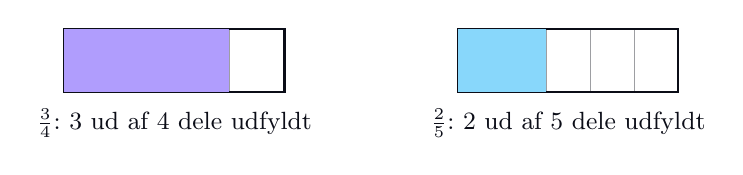
\begin{tikzpicture}
  % To visualiseringer side om side
  % Venstre: 3/4
  \begin{scope}[xshift=0cm]
    \foreach \i in {0,1,2,3} {
      \draw[bgink!40, thin] (\i*0.7,0) -- (\i*0.7,0.8);
    }
    \draw[bgink, thick] (0,0) rectangle (2.8,0.8);
    \fill[bgpurple!60] (0,0) rectangle (2.1,0.8);
    \node[bgink] at (1.4,-0.4) {\small $\tfrac{3}{4}$: 3 ud af 4 dele udfyldt};
  \end{scope}
  % Hoejre: 2/5
  \begin{scope}[xshift=5cm]
    \foreach \i in {0,1,2,3,4} {
      \draw[bgink!40, thin] (\i*0.56,0) -- (\i*0.56,0.8);
    }
    \draw[bgink, thick] (0,0) rectangle (2.8,0.8);
    \fill[bgcyan!60] (0,0) rectangle (1.12,0.8);
    \node[bgink] at (1.4,-0.4) {\small $\tfrac{2}{5}$: 2 ud af 5 dele udfyldt};
  \end{scope}
\end{tikzpicture}
\end{center}

\noindent Billedet viser to brøker som ``andel af en hel''. Den udfyldte del er brøkens værdi.

\regel{Gange brøker: tæller$\cdot$tæller over nævner$\cdot$nævner. Dividere: gang med den omvendte brøk.}{%
\textbf{Pitfall:} glem aldrig at skifte fortegn ved division med en negativ brøk: $\tfrac{a}{b}:\bigl(-\tfrac{c}{d}\bigr)=-\tfrac{a\cdot d}{b\cdot c}$.
}

\opg{Opgave 1.1}{Forkort følgende brøker mest muligt: (a) $\dfrac{8}{12}$, (b) $\dfrac{15}{25}$, (c) $\dfrac{18}{30}$.}

\opg{Opgave 1.2}{Regn ud og angiv svaret i simplest form:
\[
\frac{2}{5}+\frac{3}{4}, \qquad \frac{5}{6}-\frac{1}{3}, \qquad \frac{3}{7}+\frac{2}{7}.
\]}

\opg{Opgave 1.3}{Regn ud:
\[
\frac{2}{3}\cdot\frac{5}{8}, \qquad \frac{7}{4}\cdot\frac{3}{14}, \qquad \frac{3}{4}:\frac{5}{2}.
\]}

\opg{Opgave 1.4 (bonus)}{En opskrift på 4 personer bruger $\tfrac{2}{3}$ dl olie. Hvor meget olie skal du bruge til 6 personer, hvis mængden vokser proportionalt?}

% ===========================================================
\section{Statistik og sandsynlighed — middelværdi, median og P}
% ===========================================================

\crash{Statistik handler om at \textbf{opsummere mange tal} til ét eller to nøgletal, man kan sammenligne. Sandsynlighed handler om at \textbf{forudsige chancen} for en hændelse. Begge dele bygger på den samme idé: tæl gunstige udfald og sammenlign med det samlede antal muligheder.}

\noindent Centrale begreber:
\begin{itemize}[leftmargin=2em,itemsep=2pt]
\item \textbf{Stikprøve} (dataset): de tal vi har målt.
\item \textbf{Middelværdi (gennemsnit):} $\bar x = \dfrac{x_1+x_2+\ldots+x_n}{n}$.
\item \textbf{Median:} den midterste værdi når data er sorteret (eller gennemsnittet af de to midterste, hvis $n$ er lige).
\item \textbf{Median vs.\ middelværdi:} medianen er robust over for ekstreme værdier (outliers), middelværdien er følsom.
\item \textbf{Sandsynlighed:} $P(\text{hændelse})=\dfrac{\text{antal gunstige udfald}}{\text{antal mulige udfald}}$, når alle udfald er lige sandsynlige.
\end{itemize}

\regel{Middelværdi: læg alle tal sammen og divider med antal. Median: sortér og tag midten.}{%
\textbf{Huskeregel:} hvis der er outliers (fx én elev med karakteren 00 og resten med 7--10), så er \textbf{medianen} et bedre bud på ``det typiske'' end middelværdien.
}

\begin{center}
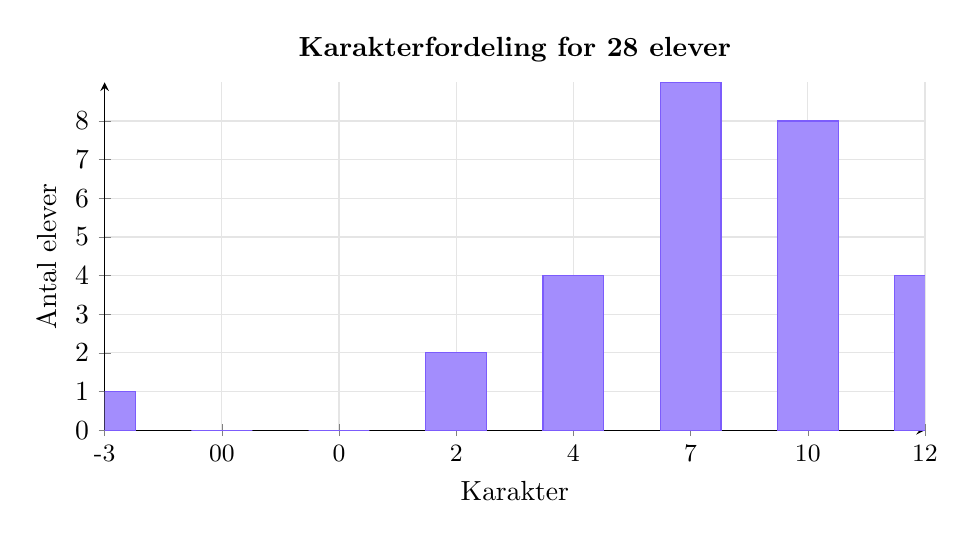
\begin{tikzpicture}
\begin{axis}[
  width=12cm, height=6cm,
  ybar,
  bar width=22pt,
  ymin=0, ymax=9,
  axis lines=left,
  symbolic x coords={-3,00,0,2,4,7,10,12},
  xtick=data,
  xlabel={Karakter}, ylabel={Antal elever},
  xticklabel style={font=\small},
  ytick={0,1,...,8},
  grid=major, grid style={gray!20},
  title={Karakterfordeling for 28 elever}, title style={font=\bfseries,yshift=-2pt}
]
\addplot[fill=bgpurple!70, draw=bgpurple] coordinates {
  (-3,1) (00,0) (0,0) (2,2) (4,4) (7,9) (10,8) (12,4)
};
\end{axis}
\end{tikzpicture}
\end{center}

\noindent Fordelingen: $-3$ (1 elev), $2$ (2), $4$ (4), $7$ (9), $10$ (8), $12$ (4). Sum: $1+2+4+9+8+4=28$ elever. De fleste ligger i den $\emptyset$vre midtergruppe (7--12). Middelværdien er $\frac{-3\cdot 1+2\cdot 2+4\cdot 4+7\cdot 9+10\cdot 8+12\cdot 4}{28}=\frac{-3+4+16+63+80+48}{28}=\frac{208}{28}\approx 7{,}4$. Medianen er den 14.--15. værdi (midten), som begge er $7$ — så median $=7$. Forskellen mellem middelværdi (7,4) og median (7) er lille, fordi $-3$ kun er én elev.

\noindent I eksemplet ovenfor er de fleste elever i den $\emptyset$vre midtergruppe (7--12). Middelværdien ($\approx 7{,}4$) er tæt på medianen ($7$), fordi $-3$-eleven kun er en enkelt outlier. Hvis vi fjernede den, ville middelværdien stige til $\tfrac{211}{27}\approx 7{,}8$ mens medianen ville være uændret — det er præcis forskellen mellem følsom og robust.

\eksempel{Middelværdi og median for $2, 5, 5, 7, 11$}{%
  Sum: $2+5+5+7+11=30$. Antal tal: $5$.\\[3pt]
  Middelværdi: $\bar x=\dfrac{30}{5}=6$.\\[3pt]
  Median: data er allerede sorteret, den midterste (3.\,største) er $\mathbf{5}$.\\[3pt]
  \textit{Bemærk:} middelværdien (6) er større end medianen (5), fordi 11 trækker op. Medianen er et bedre bud på ``det typiske tal'' her.
}

\eksempel{Sandsynlighed for en bestemt terning}{%
  En almindelig terning har 6 sider, alle lige sandsynlige.\\[3pt]
  $P(\text{slå et 4-tal})=\dfrac{1}{6}\approx 16{,}7\%$.\\[3pt]
  $P(\text{slå et lige tal})=\dfrac{3}{6}=\dfrac{1}{2}=50\%$ (udfald: 2, 4, 6).\\[3pt]
  \textit{Fortolkning:} ``lige tal'' rummer 3 ud af 6 muligheder, så sandsynligheden er 50\%.
}

\eksempel{To terningekast — hvad er $P(\text{to 6'ere})$?}{%
  Kast 1: $P(6)=\tfrac{1}{6}$. Kast 2: $P(6)=\tfrac{1}{6}$ (uafhængige kast).\\[3pt]
  $P(\text{begge}=6)=\tfrac{1}{6}\cdot\tfrac{1}{6}=\tfrac{1}{36}\approx 2{,}8\%$.\\[3pt]
  \textit{Regel:} uafhængige hændelser ganges. ``Uafhængig'' betyder at det ene kast ikke påvirker det andet.
}

\opg{Opgave 2.1}{Beregn middelværdi og median for datasættet: $3, 7, 7, 2, 9, 4, 7, 1, 8$.}

\opg{Opgave 2.2}{I en klasse på 24 elever er der 14 piger og 10 drenge. Hvad er sandsynligheden for tilfældigt at udtrække (a) en pige, (b) en dreng, (c) en elev der enten er pige eller dreng?}

\opg{Opgave 2.3}{Du kaster to terninger. Hvad er sandsynligheden for at summen af de to øjne er (a) 7, (b) højst 4, (c) præcis 12? Tip: lav en tabel over alle 36 udfald.}

\opg{Opgave 2.4 (bonus)}{En urne indeholder 3 røde, 5 blå og 2 grønne kugler. Du trækker én kugle tilfældigt. Hvad er sandsynligheden for (a) rød, (b) ikke-grøn, (c) gul? Hvad er den samlede sandsynlighed for alle tre farver?}

% ===========================================================
\section{Trigonometri — retvinklede trekanter}
% ===========================================================

\crash{Trigonometri handler om \textbf{forholdet mellem siderne} i en retvinklet trekant. Vi definerer tre funktioner — $\sin$, $\cos$ og $\tan$ — der kun afhænger af \emph{en af de to ikke-rette vinkler}. Det er det smukke: samme trekant, uanset størrelse, har samme forhold mellem siderne, hvis vinklen er den samme.}

\noindent Enhedscirklen er en cirkel med radius 1. For en vinkel $\theta$ målt fra den positive $x$-akse:
\begin{itemize}[leftmargin=2em,itemsep=2pt]
\item $\cos\theta$ er $x$-koordinaten for punktet på cirklen.
\item $\sin\theta$ er $y$-koordinaten for punktet på cirklen.
\item $\tan\theta=\dfrac{\sin\theta}{\cos\theta}$.
\end{itemize}

\noindent For en \textbf{retvinklet trekant} med en af de spidse vinkler lig $\theta$:
\begin{itemize}[leftmargin=2em,itemsep=2pt]
\item \textbf{Hypotenuse:} siden overfor den rette vinkel (længste side).
\item \textbf{Modstående katete:} siden overfor vinklen $\theta$.
\item \textbf{Hosliggende katete:} siden ved siden af $\theta$ (og ikke hypotenusen).
\end{itemize}

\regel{Definitioner (huskes på remse: \textbf{H}os \textbf{M}od $\Rightarrow$ \textbf{HM} for $\cos$ og $\sin$):}{%
\[
\sin\theta=\frac{\text{modstående}}{\text{hypotenuse}}, \qquad
\cos\theta=\frac{\text{hosliggende}}{\text{hypotenuse}}, \qquad
\tan\theta=\frac{\text{modstående}}{\text{hosliggende}}.
\]
}

\begin{center}
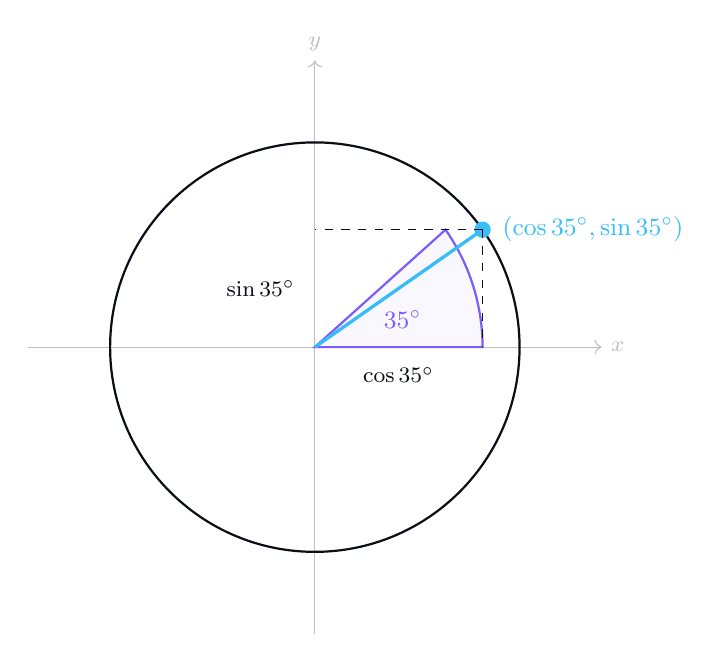
\begin{tikzpicture}[scale=2.6]
  % Cirkel
  \draw[->,gray!50,thin] (-1.4,0) -- (1.4,0) node[right,font=\footnotesize]{$x$};
  \draw[->,gray!50,thin] (0,-1.4) -- (0,1.4) node[above,font=\footnotesize]{$y$};
  \draw[bgink, thick] (0,0) circle (1);
  % Vinkel på 35 grader
  \def\ang{35}
  \fill[bgpurple!15, draw=bgpurple, thick, fill opacity=0.3] (0,0) -- ({cos(\ang)},0) arc (0:\ang:1) -- cycle;
  \draw[bgcyan, very thick] (0,0) -- ({cos(\ang)},{sin(\ang)});
  \fill[bgcyan] ({cos(\ang)},{sin(\ang)}) circle (0.04);
  \node[bgcyan, anchor=west] at ({cos(\ang)+0.05},{sin(\ang)}) {\small$(\cos 35^\circ,\sin 35^\circ)$};
  \node[bgpurple, font=\small] at ({0.45*cos(\ang/2)},{0.45*sin(\ang/2)}) {$35^\circ$};
  \draw[bgink, dashed, thin] ({cos(\ang)},{sin(\ang)}) -- ({cos(\ang)},0);
  \draw[bgink, dashed, thin] ({cos(\ang)},{sin(\ang)}) -- (0,{sin(\ang)});
  \node[bgink, font=\footnotesize, below] at ({cos(\ang)/2},-0.05) {$\cos 35^\circ$};
  \node[bgink, font=\footnotesize, left] at (-0.05,{sin(\ang)/2}) {$\sin 35^\circ$};
\end{tikzpicture}
\end{center}

\noindent På enhedscirklen er radius 1, så punktet $(\cos\theta,\sin\theta)$ sidder lige præcis på cirklen. Det er den geometriske definition af $\cos$ og $\sin$.

\eksempel{En retvinklet trekant med vinkler 30, 60, 90 og hypotenuse 10}{%
  Modstående katete til 30$^\circ$: $10\cdot\sin 30^\circ=10\cdot 0{,}5=5$.\\[3pt]
  Hosliggende katete til 30$^\circ$: $10\cdot\cos 30^\circ=10\cdot 0{,}866\approx 8{,}66$.\\[3pt]
  \textit{Tjek:} $5^2+8{,}66^2=25+75=100=10^2$ — Pythagoras holder.
}

\eksempel{Stigen op ad en mur}{%
  En stige på 4\,m står op ad en lodret mur og danner vinklen 70$^\circ$ med jorden. Hvor højt op rør stigen muren?\\[3pt]
  Stigen er hypotenusen (4\,m). Den lodrette side er \textbf{modstående} til 70$^\circ$.\\[3pt]
  $\sin 70^\circ=\dfrac{\text{modstående}}{\text{hypotenuse}}=\dfrac{h}{4}$.\\[3pt]
  $h=4\cdot\sin 70^\circ\approx 4\cdot 0{,}9397\approx 3{,}76$\,m.\\[3pt]
  \textit{Tolkning:} stigen rør muren i ca.\ 3,76 meters højde.
}

\eksempel{Bestem vinklen i en trekant med kateter 3 og 5}{%
  Vi har en retvinklet trekant, den hosliggende katete (til vinklen) er 3, den modstående er 5.\\[3pt]
  $\tan\theta=\dfrac{5}{3}\approx 1{,}667$.\\[3pt]
  $\theta=\tan^{-1}(1{,}667)\approx 59{,}0^\circ$.\\[3pt]
  \textit{Tjek:} Pythagoras giver hypotenusen $\sqrt{3^2+5^2}=\sqrt{34}\approx 5{,}83$.
}

\opg{Opgave 3.1}{I en retvinklet trekant er den hosliggende katete 8 og hypotenusen 17. Beregn (a) $\cos\theta$, (b) $\sin\theta$, (c) $\tan\theta$.}

\opg{Opgave 3.2}{En mand ser op på toppen af en bygning. Han står 30\,m fra bygningens fod, og hans synslinje danner vinklen 35$^\circ$ med vandret. Hvor høj er bygningen?}

\opg{Opgave 3.3}{En flyvemaskine letter i en vinkel på 12$^\circ$ med vandret. Efter 500\,m langs flyveretningen, hvor højt er den? Tip: hypotenusen er 500\,m.}

\opg{Opgave 3.4 (bonus)}{En retvinklet trekant har siderne 5, 12 og 13. Find alle tre spidse vinkler (i grader, afrundet til én decimal). Tip: start med den mindste vinkel.}

% ===========================================================
\newpage
\section*{Appendix — Facit}
% ===========================================================

\f{1.1}{(a) $\dfrac{8}{12}=\dfrac{8:4}{12:4}=\dfrac{2}{3}$. \quad (b) $\dfrac{15}{25}=\dfrac{15:5}{25:5}=\dfrac{3}{5}$. \quad (c) $\dfrac{18}{30}=\dfrac{18:6}{30:6}=\dfrac{3}{5}$.}

\f{1.2}{$\tfrac{2}{5}+\tfrac{3}{4}$: fællesnævner 20. $\tfrac{8}{20}+\tfrac{15}{20}=\tfrac{23}{20}=1\tfrac{3}{20}$.\\[2pt]
$\tfrac{5}{6}-\tfrac{1}{3}=\tfrac{5}{6}-\tfrac{2}{6}=\tfrac{3}{6}=\tfrac{1}{2}$.\\[2pt]
$\tfrac{3}{7}+\tfrac{2}{7}=\tfrac{5}{7}$ (allerede samme nævner).}

\f{1.3}{$\tfrac{2}{3}\cdot\tfrac{5}{8}=\tfrac{10}{24}=\tfrac{5}{12}$.\\[2pt]
$\tfrac{7}{4}\cdot\tfrac{3}{14}=\tfrac{21}{56}=\tfrac{3}{8}$ (divider med 7).\\[2pt]
$\tfrac{3}{4}:\tfrac{5}{2}=\tfrac{3}{4}\cdot\tfrac{2}{5}=\tfrac{6}{20}=\tfrac{3}{10}$.}

\f{1.4}{Forholdet mellem personer: $\tfrac{6}{4}=\tfrac{3}{2}=1{,}5$. Så olie $=1{,}5\cdot\tfrac{2}{3}\text{ dl}=\tfrac{3}{3}\text{ dl}=1\text{ dl}$.}

\f{2.1}{Sorteret: $1, 2, 3, 4, 7, 7, 7, 8, 9$. Sum $=48$, $n=9$.\\[2pt]
Middelværdi: $\bar x=\tfrac{48}{9}\approx 5{,}33$.\\[2pt]
Median: 5.\,værdi (midten) $=7$.\\[2pt]
\textit{Bemærk:} middelværdien er lavere end medianen, fordi 1 og 2 trækker ned.}

\f{2.2}{(a) $P(\text{pige})=\tfrac{14}{24}=\tfrac{7}{12}\approx 58{,}3\%$.\\[2pt]
(b) $P(\text{dreng})=\tfrac{10}{24}=\tfrac{5}{12}\approx 41{,}7\%$.\\[2pt]
(c) $P(\text{pige eller dreng})=\tfrac{24}{24}=1$ (sikker hændelse).}

\f{2.3}{Mulige summer: $2$ (1 komb.), $3$ (2), $4$ (3), $5$ (4), $6$ (5), $7$ (6), $8$ (5), $9$ (4), $10$ (3), $11$ (2), $12$ (1). I alt 36.\\[2pt]
(a) $P(7)=\tfrac{6}{36}=\tfrac{1}{6}\approx 16{,}7\%$.\\[2pt]
(b) $P(\leq 4)=\tfrac{1+2+3}{36}=\tfrac{6}{36}=\tfrac{1}{6}\approx 16{,}7\%$.\\[2pt]
(c) $P(12)=\tfrac{1}{36}\approx 2{,}8\%$.}

\f{2.4}{Total: $3+5+2=10$ kugler.\\[2pt]
(a) $P(\text{rød})=\tfrac{3}{10}=30\%$.\\[2pt]
(b) $P(\text{ikke-grøn})=\tfrac{8}{10}=80\%$.\\[2pt]
(c) $P(\text{gul})=0$ (ingen gule kugler i urnen).\\[2pt]
Total $P$ for de tre farver: $P(\text{rød})+P(\text{blå})+P(\text{grøn})=30\%+50\%+20\%=100\%$ — alle udfald dækket.}

\f{3.1}{Hosliggende 8, hypotenuse 17.\\[2pt]
(a) $\cos\theta=\tfrac{8}{17}\approx 0{,}4706$.\\[2pt]
(b) Pythagoras: modstående $=\sqrt{17^2-8^2}=\sqrt{289-64}=\sqrt{225}=15$. $\sin\theta=\tfrac{15}{17}\approx 0{,}8824$.\\[2pt]
(c) $\tan\theta=\tfrac{15}{8}=1{,}875$.}

\f{3.2}{Den lodrette side er modstående, den vandrette (30\,m) er hosliggende, men vi kender afstand + vinklen med vandret.\\[2pt]
$\tan 35^\circ=\dfrac{h}{30}\Rightarrow h=30\cdot\tan 35^\circ\approx 30\cdot 0{,}7002\approx 21{,}0$\,m.\\[2pt]
\textit{Tjek med $\sin$:} afstand til toppunkt $=\tfrac{30}{\cos 35^\circ}\approx 36{,}6$\,m, og $36{,}6\cdot\sin 35^\circ\approx 21{,}0$\,m — samme resultat.}

\f{3.3}{Hypotenuse 500\,m, vinkel 12$^\circ$ med vandret. Den lodrette højde er modstående.\\[2pt]
$h=500\cdot\sin 12^\circ\approx 500\cdot 0{,}2079\approx 104{,}0$\,m.\\[2pt]
\textit{Bemærk:} det er en flad vinkel, så flyet er ikke så højt som man måske tror — kun ca.\ 100\,m op efter en halv kilometer.}

\f{3.4}{Sider: 5, 12, 13. Hypotenuse 13.\\[2pt]
Lille vinkel (modstående 5): $\sin\theta_1=\tfrac{5}{13}\Rightarrow\theta_1=\sin^{-1}(\tfrac{5}{13})\approx 22{,}6^\circ$.\\[2pt]
Stor vinkel (modstående 12): $\theta_2=\sin^{-1}(\tfrac{12}{13})\approx 67{,}4^\circ$.\\[2pt]
Tjek: $22{,}6^\circ+67{,}4^\circ+90^\circ=180^\circ$ — sum af vinkler i trekant.}

\end{document}
